\chapter{Fibre Bundles}\label{chapter:bundles}

    This chapter is formulated in sufficient generality so as to encompass both the topological and smooth setting (or any other setting one might find useful). To this end, the generic terms `space', `group' and `morphism' are used. The reader should choose in which category to work, e.g.~topological space, topological group and continuous map in the case of $\mathbf{Top}$.

    \minitoc

\section{Bundles}

    \newdef{Bundle}{\index{bundle}\label{bundle:bundle}
        A triple $(E,B,\pi)$ where $E$ and $B$ are spaces and $\pi:E\rightarrow B$ is a morphism. Sometimes, $\pi$ is required to be surjective. However, under this additional restriction, one cannot make the association $\mathbf{Bundle}(B)\cong\mathbf{C}_{/B}$ of categories.
    }

    An explicit example in the category $\mathbf{Diff}$ is the following.
    \begin{example}[Fibred manifold]\index{fibred!manifold}\index{fibre}
        A surjective submersion (\cref{manifold:submersion}) \[\pi:E\rightarrow B,\] where $E$ is called the \textbf{total space}, $B$ the \textbf{base space} and $\pi$ the \textbf{projection}. For every point $p\in B$, the set $\pi^{-1}(p)$ is called the \textbf{fibre over $p$}.
    \end{example}

    The most important example of a bundle is a fibre bundle. Before being able to give the definition, an important concept needs to be introduced.
    \newdef{Cocycle}{\index{co-!cycle}\label{bundle:G_cocycle}
        Let $B$ be a space and $G$ a group. A $G$-valued cocycle on $B$ with respect to an open cover $\{U_i\}_{i\in I}$ is a family of morphisms $g_{ij}:U_i\cap U_j\rightarrow G$ that satisfy the \textbf{\v{C}ech cocycle condition}
        \begin{gather}
            \label{bundle:G_cocycle_condition}
            g_{ij} = g_{ik}\circ g_{kj}
        \end{gather}
        for all $i,j,k\in I$. Two cocycles $(U_i,g_{ij})$ and $(V_i,h_{ij})$ are said to be equivalent if there exist morphisms $\lambda_{i,j}:U_i\cap V_j\rightarrow G$ such that
        \begin{gather}
            \lambda_{i,r}g_{ij}\lambda_{j,s}^{-1} = h_{rs}
        \end{gather}
        whenever this is well defined. The resulting quotient set is denoted by $\check{H}^1(B;G)$.\footnote{The notation stems from the fact that this is the first \v{C}ech cohomology group with values in $G$ (\cref{section:cech}).}
    }
    \begin{property}[Normalization]\label{bundle:G_cocycle_conditions}
        Let $\{g_{ij}\}_{i,j\in I}$ be a cocycle on $B$. It satisfies the following properties for all $x\in B$:
        \begin{itemize}
            \item $g_{ij}(x) = g_{ji}(x)^{-1}$, and
            \item $g_{ii}(x) = e$.
        \end{itemize}
    \end{property}

    \newdef{Fibre bundle}{\index{fibre!bundle}\index{local!trivialization}\index{structure!group}\label{bundle:fibre_bundle}
        A tuple $(E,B,\pi,F,G)$ where $E,B$ and $F$ are spaces and $G$ is a group, called the \textbf{structure group}, such that there exists a surjective morphism \[\pi:E\rightarrow B\] and an open cover $\{U_i\}_{i\in I}$ of $B$ together with a family of isomorphisms $\{\varphi_i:\pi^{-1}(U_i)\rightarrow U_i\times F\}_{i\in I}$ that make the following diagram commute for all $i\in I$:
        \begin{gather*}
            \centering
            \begin{tikzpicture}
                \node (PI) at (-2, 0) {$\pi^{-1}(U_i)$};
                \node (UF) at (2, 0) {$U_i\times F$};
                \node (U) at (0, -2) {$U_i$};
                \draw[->] (PI) -- node[above]{$\varphi_i$} (UF);
                \draw[->] (PI) -- node[below left]{$\pi$} (U);
                \draw[->] (UF) -- node[below right]{$\pr_1$} (U);
            \end{tikzpicture}
        \end{gather*}
        As for general bundles, one calls $E$ and $B$ the \textbf{total space} and \textbf{base space}, respectively. The space $F$ is called the \textbf{(typical) fibre}. The pair $(U_i,\varphi_i)$ is sometimes called a \textbf{bundle chart} and the set $\{(U_i,\varphi_i)\}_{i\in I}$ is often called a \textbf{local trivialization}\footnote{This terminology follows from the fact that the bundle is locally isomorphic to a (trivial) product space: $E\cong U\times F$.}. The cover $\{U_i\}_{i\in I}$ itself is called a \textbf{trivializing cover} of the bundle.

        The \textbf{transition maps} $\varphi_j\circ\varphi_i^{-1}:(U_i\cap U_j)\times F\rightarrow (U_i\cap U_j)\times F$ can be identified with a cocycle $g_{ji}:U_i\cap U_j\rightarrow G$ as follows. The transition maps restrict to the identity on $B$ and, hence, act only on the fibres:
        \begin{gather}
            \varphi_j\circ\varphi_i^{-1}(b,x) = \bigl(b,g_{ji}(b)\cdot x\bigr)\,.
        \end{gather}
        The compatibility conditions satisfied by the functions $g_{ji}$, obtained by considering triple intersections, are exactly the cocycle conditions~\eqref{bundle:G_cocycle_condition}. Moreover, it can be shown that this action of $G$ on every fibre is faithful (\cref{group:faithful_action}).
    }
    \begin{remark}
        One should pay attention to the fact that the bundle charts are not coordinate charts in the sense of manifolds (\cref{manifold:chart}), because the image of $\varphi_i$ is not an open subset of $\mathbb{R}^n$. However, they serve the same purpose as they are used to locally describe the total space $P$.
    \end{remark}
    \begin{notation}
        A fibre bundle $(E,B,\pi,F,G)$ is often denoted by $F\hookrightarrow E\overset{\pi}{\rightarrow}{B}$ or even by the morphism $\pi:E\rightarrow B$ if the fibre is not important. A drawback of such notations is that the structure group of the bundle is not immediately clear.
    \end{notation}

    \newdef{Numerable fibre bundle}{\index{numerable}\label{bundle:numerable_bundle}
        A fibre bundle that admits a local trivialization over a numerable open cover (\cref{topology:numerable_cover}).
    }

    \newdef{Compatible bundle charts}{\index{admissible}\index{bundle}
        A bundle chart $(V,\psi)$ is said to be \textbf{admissible} or compatible with a trivializing cover $\{(U_i,\varphi_i)\}_{i\in I}$ if, whenever $V\cap U_i\neq\emptyset$, there exists a map $h_i:V\cap U_i\rightarrow G$ such that
        \begin{gather}
            \psi\circ\varphi_i^{-1}(b,x) = \bigl(b,h_i(b)x\bigr)
        \end{gather}
        for all $b\in V\cap U_i$ and $x\in F$. Two trivializing covers are said to be equivalent if all bundle charts are mutually compatible. As in the case of manifolds, this gives rise to the notion of a \textbf{$G$-atlas}. A \textbf{$G$-bundle} is then defined as a fibre bundle equipped with an equivalence class of $G$-atlases.
    }

    \newdef{Bundle map}{\index{bundle!map}\label{bundle:bundle_map}
        A bundle map between two fibre bundles $\pi_1:E_1\rightarrow B_1$ and $\pi_2:E_2\rightarrow B_2$ is a pair $(f_E,f_B)$ of morphisms that make Diagram~\ref{fig:bundle_map} commute. The map $f_E$ is said to \textbf{cover} $f_B$. If such a couple exists, the base map $f_B$ is uniquely determined by $f_E$ and, therefore, a bundle map is often just denoted by $f_E:E_1\rightarrow E_2$.
    }

    \begin{figure}[ht!]
        \centering
        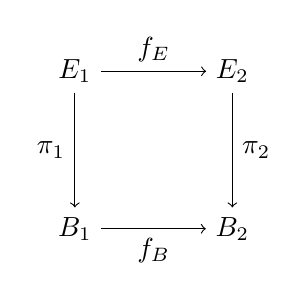
\begin{tikzpicture}
            \node (E1) at (0, 0) {$E_1$};
            \node (E2) at (2, 0) {$E_2$};
            \node (B1) at (0, -2) {$B_1$};
            \node (B2) at (2, -2) {$B_2$};
            \draw[->] (E1) -- node[above]{$f_E$} (E2);
            \draw[->] (E1) -- node[left]{$\pi_1$} (B1);
            \draw[->] (E2) -- node[right]{$\pi_2$} (B2);
            \draw[->] (B1) -- node[below]{$f_B$} (B2);
        \end{tikzpicture}
        \caption{Bundle map between fibre bundles.}
        \label{fig:bundle_map}
    \end{figure}

    \newdef{Equivalent fibre bundles}{\index{gauge!transformation}
        Two fibre bundles $\pi_1:E_1\rightarrow B$ and $\pi_2:E_2\rightarrow B$ with the same typical fibre and structure group are said to be equivalent if there exist trivializations $\{(U_i,\varphi_i)\}_{i\in I}$ and $\{(U_i,\varphi'_i)\}_{i\in I}$ such that the associated cocycles are equivalent (note that the cover $\{U_i\}_{i\in I}$ is the same for both trivializations). An explicit form of the functions $\lambda$ is given by
        \begin{gather}
            \lambda_i := \varphi_i'\circ\varphi_i^{-1}\,.
        \end{gather}
    }
    \begin{property}[Isomorphism]
        Two fibre bundles over the same base space are equivalent if and only if they are isomorphic.
    \end{property}

    \newdef{Trivial bundle}{\index{trivial}\label{bundle:trivial_bundle}
        A fibre bundle $(E,B,\pi,F)$ is said to be trivial if there exists an equivalence $E\cong B\times F$.
    }

\section{Constructions}

    \begin{construct}[Construction theorem\footnotemark]\index{clutching}\label{bundle:fibre_bundle_construction_theorem}
        \footnotetext{Sometimes also called the \textbf{clutching theorem}. See further one for an explanation.}
        Let $B$ and $F$ be spaces and let $G$ be a group equipped with a faithful (left) action on $F$. Suppose that a cover $\{U_i\}_{i\in I}$ of $B$ and a collection of morphisms $\{g_{ji}:U_i\cap U_j\rightarrow G\}$ that satisfy the cocycle condition~\eqref{bundle:G_cocycle} are given. A fibre bundle over $B$ can be constructed as follows:
        \begin{enumerate}
            \item Construct, for every set $U_i$, the Cartesian product $U_i\times F$.
            \item Construct the disjoint union $\bigsqcup_{i\in I}U_i\times F$ and equip it with the disjoint union topology (\cref{topology:disjoint_union}).
            \item From this disjoint union, construct a quotient space, equipped with the quotient space topology (\cref{topology:quotient_space}), induced by the following equivalence relations for all $i,j\in I$:
                \begin{gather}
                    (b,f)\sim\bigl(b,g_{ji}(b)\cdot f\bigr)\,,
                \end{gather}
                where $b\in U_i\cap U_j$ and $f\in F$ (note that the disjoint union indices are suppressed in this notation).
        \end{enumerate}
        The fibre bundle $E$ is equal to this quotient space, where $\pi:E\rightarrow B:[(b,f)]\mapsto b$ is the quotient space projection. Local trivializations are given by the maps $\varphi_i:\pi^{-1}(U_i)\rightarrow U_i\times F$ that satisfy
        \begin{gather}
            \varphi_i^{-1}:(b,f)\mapsto[(b,f)]\,.
        \end{gather}
    \end{construct}
    \begin{remark}[Topology]
        Although the resulting fibre bundle is, by construction, bijective (as a set) to the Cartesian product $B\times F$ or the disjoint union $\bigsqcup_{b\in B}F$, this does not hold on the level of topologies. It is not equipped with the disjoint union topology!
    \end{remark}

    \begin{property}[Homotopy invariance]
        Homotopic transition functions give rise to equivalent bundles.
    \end{property}

    \begin{remark}[Clutching]\index{clutching}\label{bundle:clutching_theorem}
        The above construction is often called the \textbf{clutching construction}, especially when constructing vector bundles over a (hyper)sphere $S^n$. In that case, the covering consists of two hemispheres that intersect on the equator $S^{n-1}$ and the function $g_{21}$ is called the \textbf{clutching function}.
    \end{remark}

    \begin{construct}[Pullback bundle]\index{pullback!of a bundle}\label{bundle:pullback_bundle}
        Let $\pi:E\rightarrow B$ be a fibre bundle and let $f:B'\rightarrow B$ be a morphism of spaces. The pullback (\cref{cat:pullback}) of $\pi$ and $f$ gives the total space of the pullback bundle $f^*E$:
        \begin{gather}
            f^*E := \bigl\{(b',e)\in B'\times E\bigm\vert f(b') = \pi(e)\bigr\}\,.
        \end{gather}
        The topology on $f^*E$ is induced by the subspace topology of $B'\times E$. The projection onto the second factor gives a map of total spaces $f^*E\rightarrow E$.
    \end{construct}

    \begin{construct}[Fibre product]\index{fibre!product}\label{bundle:fibre_product}
        Let $(E_1,B,\pi_1)$ and $(E_2,B,\pi_2)$  be two fibre bundles over the same base space $B$. Their fibre product is defined as follows:
        \begin{gather}
            E_1\times_BE_2 := \bigl\{(p,q)\in E_1\times E_2\bigm\vert\pi_1(p) = \pi_2(q)\bigr\}\,.
        \end{gather}
        It is the pullback of one bundle along another.
    \end{construct}

\section{Sections}

    \newdef{Section}{\index{section!of a bundle}
        A (\textbf{global}) section of a fibre bundle $\pi:E\rightarrow B$ is a morphism $s:B\rightarrow E$ such that $\pi\circ s=\mathbbm{1}_B$, i.e.~a section of $\pi$ in the sense of \cref{cat:retract}. For any open subset $U\subset B$, a \textbf{local} section is defined as a morphism $s_U:U\rightarrow E$ such that $\pi\circ s_U=\mathbbm{1}_U$.
    }
    \begin{notation}
        The set of all global sections of a bundle $E$ is denoted by $\Gamma(E)$. The set of local sections over $U$ is sometimes denoted by $\Gamma(U,E)$. With this latter notation, one also has $\Gamma(E)=\Gamma(B,E)$.
    \end{notation}

    \begin{property}[Pullback of sections]
        Consider a fibre bundle $\pi:E\rightarrow B$ together with a morphism of spaces $f:B'\rightarrow B$. The sections of $E$ pullback to the pullback bundle $f^*E$ by defining $f^*s := s\circ f$.
    \end{property}